% ===============================================================================
\section{Overview}
\wingj is an open-source image processing toolkit for unsupervised, multi-scale quantification of biological systems (organ systems or body systems) \autocite{schaffter2013}. \wingj provides tools for automatic structure detection from confocal fluorescence images, which consists in generating a parametric model that accurately describes the morphology of an organ system (e.g. \droso wing pouch) or body system (e.g. \droso embryo). The approach we developed is based on the design of many \emph{detection modules} that each takes care of identifying a specific feature of the overall structure to model (\figref{fig:wingj_wpouch_detection_modules_intro}). This includes the detection and modelling of fluorescence patterns including the detection of compartments, the identification of the trajectory of fluorescence boundaries, etc. A consistent parametric model of the overall structure to quantify is then generated by integrating the outputs of the different detection modules..\\

% This \textit{structure model} provides a mean to quantify the morphology or structure of a biological system of interest. For example, one can then measure the length of the anterior/posterior (A/P) and dorsal/ventral (D/V) boundaries, and the perimeter and area of different compartments. Measurements are converted in \wingj from pixel unit to physical units (e.g. \mum and \mumsquare) using meta-information included by the microscopes in the input images.

% In \wingj, the structure detection refers to a sequence of \textit{detection modules} applied to identify specific features of the overall structure to model \citep{schaffter2013}. In the detection of the \textit{Drosophila} wing pouch structure for instance, one of the first module applied identifies where the anterior/posterior (A/P) and dorsal/ventral (D/V) boundaries intersect. Yet another module applies active contour algorithms, also called \textit{snakes} \citep{McInerney1996,DelgadoGonzalo2010a}, to segment the four compartments DA, DP, VA, and VP that are included in the wing pouch. A parametric model of the structure is then generated by combining the different output of the detection modules. We developed and implemented as much as eight detection modules to identify the wing pouch structure \citep{schaffter2013}, whose respective output is shown in Figure~\ref{fig:wingj_wpouch_detection_modules_intro}.\\

\begin{figure}[!h]
\centering
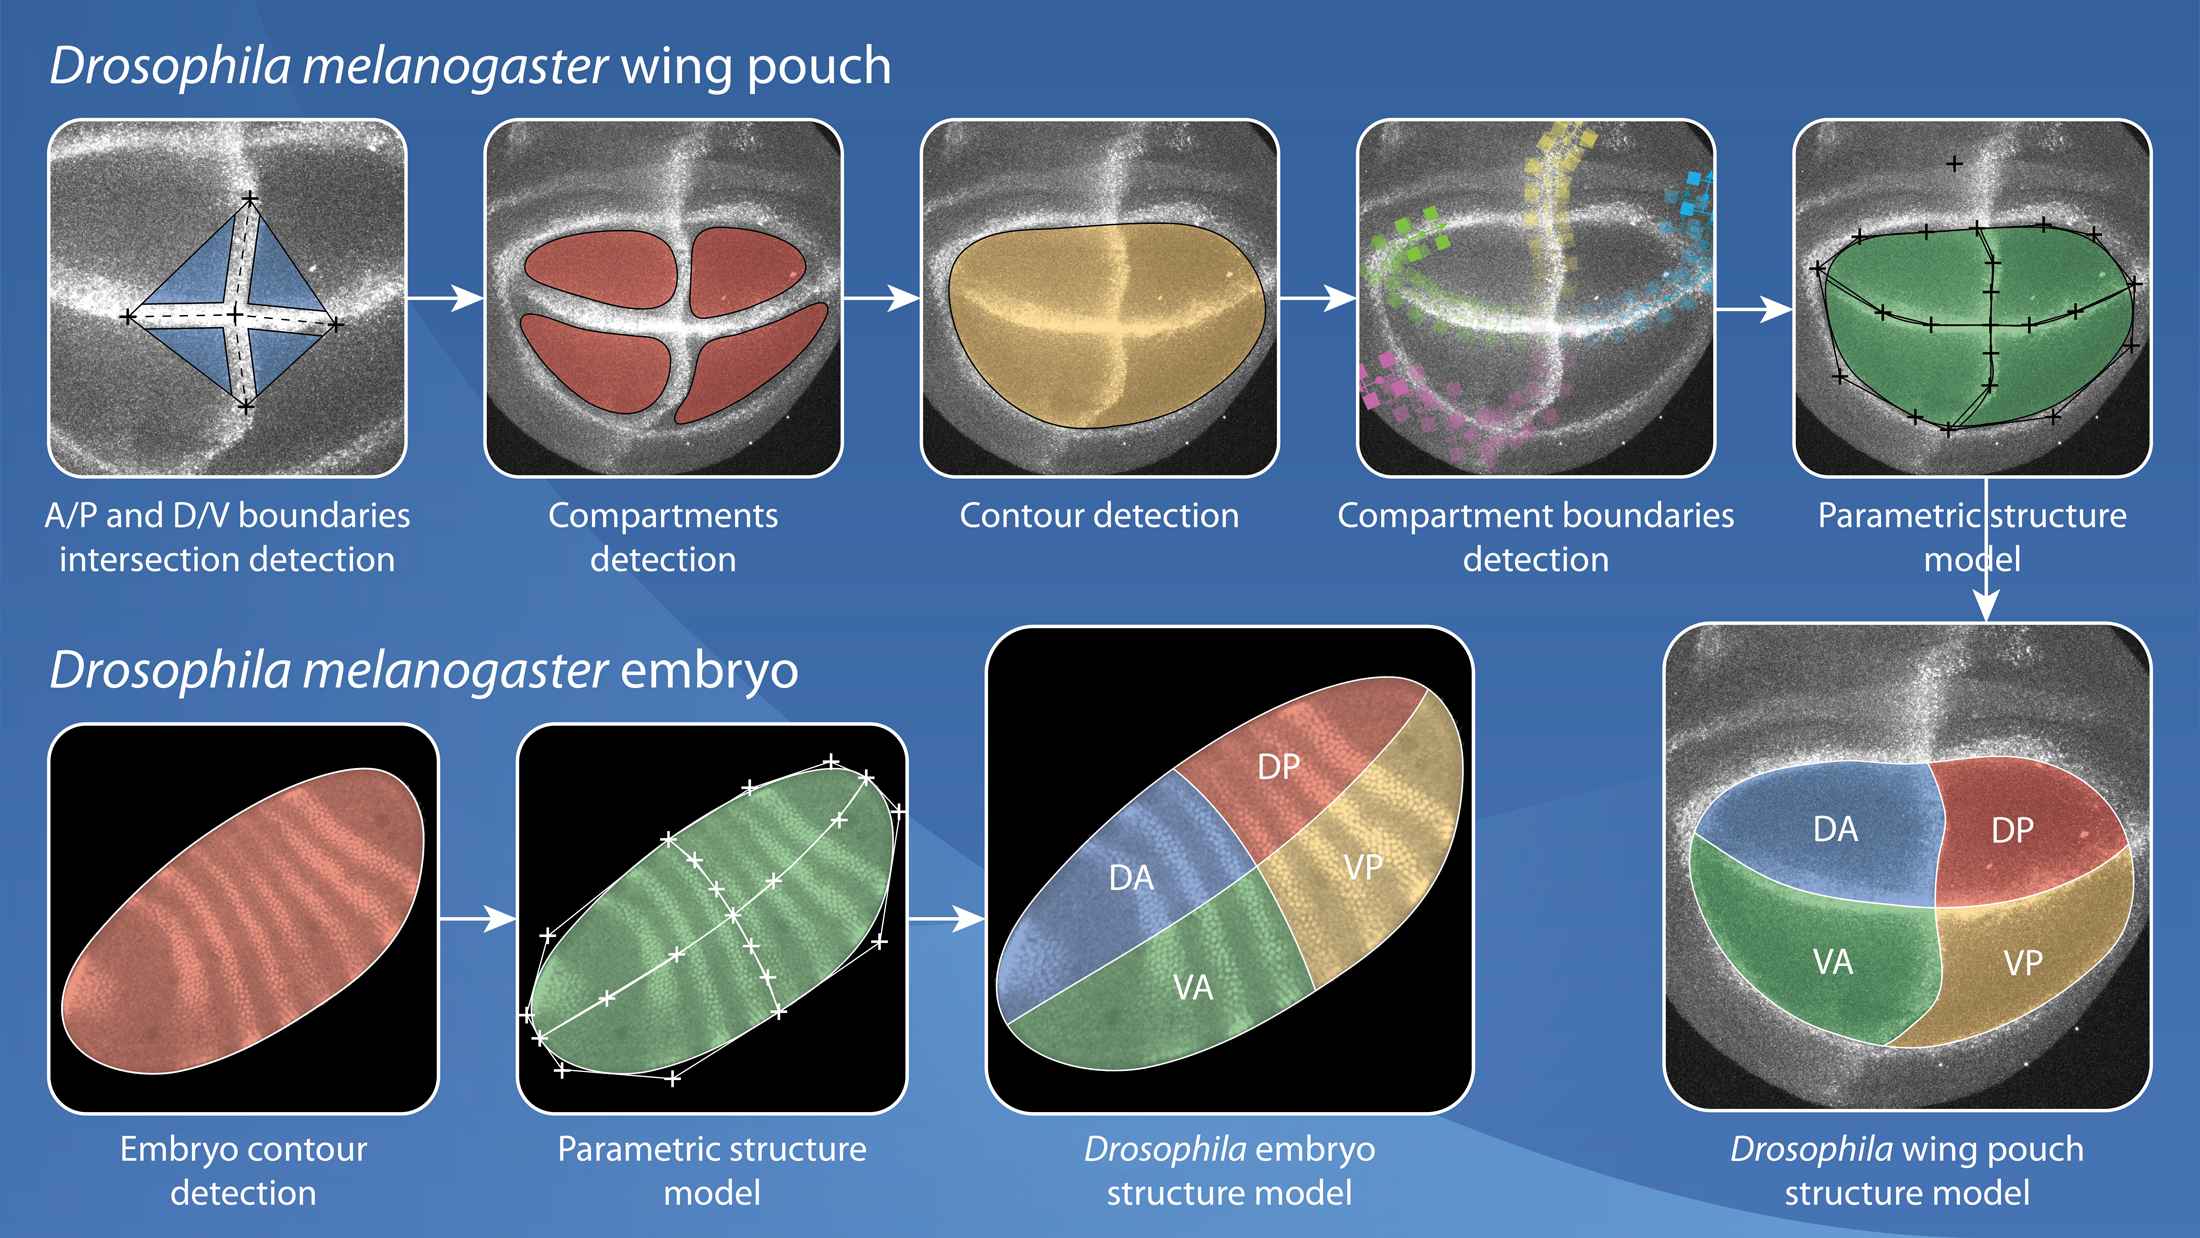
\includegraphics[width=146mm]{images/generic-diagram_300dpi.jpg} % 0.3
\caption{\textbf{Unsupervised inference of a structure models of biological systems from stacks of confocal images.} The structure detection consists in applying many \textit{detection modules} to identify different features of the structure. Here we show the different detection modules we developed to quantify the morphology or structure of the \droso wing pouch and \droso embryo. The outputs of the modules are then integrated to generate a consistent parametric model of the overall structure to describe.}
\label{fig:wingj_wpouch_detection_modules_intro}
\end{figure}

Once a structure model has been inferred, additional tools also available in \wingj to enable the quantification of expression in the space of the structure model. Different approaches are proposed to measure expression including the generation of expression profiles and \textit{expression maps}.\\

Moreover, we developed an automatic 3D cell nuclei detection method to evaluate the number of nuclei in the space defined by the structure model previously inferred using \wingj. This method takes as input a stack of confocal images where nuclei are stained, for instance using nuclear staining such as TO-PRO \autocite{suzuki1997dna} or histone GFP constructs \autocite{kanda1998histone}.\\

\sectionref{chap:getting_started} explains how to launch \wingj and how to load stacks of confocal fluorescence images. \sectionref{chap:convention} introduces a few conventions defined in \wingj which are required to achieve high level of automation, thus making \wingj easier to use and allowing to spend less time on repetitive and laborious processes. Note that scripts are also provided to automate the generation of datasets for many experiments. \sectionref{chap:structure} describes how to generate a parametric model describing accurately the structure or morphology of a biological organ system or body system. \sectionref{chap:expression} gives detailed guidelines to systematically and accurately quantify gene and protein expression in the space defined by a structure model previously inferred. \sectionref{chap:matlab} introduces the \wingjMatlab which provides tools to generate statistics and plots from the files generated by \wingj. This toolbox also implements the automatic 3D cell nuclei detection method. Finally, \sectionref{chap:protocols} summarizes the information introduced in details in the previous chapters to provide concise instructions for quantifying structure and expression information from a biological system using the tools available in \wingj.


% the methods implemented in \wingj to quantify both structure and expression information are completed by an automatic nuclei detection method. This method is released as part of the \textit{WingJ Matlab toolbox}


%  that, when combined with a structure model previously inferred, returns the number of nuclei included in the system of interest (here the structure model is used to define a subspace inside the 3D image space).\\
% 
% Users can interact with the structure model identified and edit its shape if required by moving around \textit{control points}, which provide a visual representation of the parameters of the model. Finally, the orientation of the structure model (A/P and D/V directions) is automatically inferred based on \textit{a priori} knowledge about the geometry of the wing pouch. Thus, the orientation inference is achieved independently of the orientation of the wing in the XY space of the stack of images.\\
% 
% % Therefore wings is achieved so that wings are not required to be perfectly aligned with the borders of the images.\\
% 
% Chapter~\ref{chap:getting_started} explains how to launch \wingj and how to give it access to more memory that initially allowed by Java Web Start. This is required to import large stacks of confocal images in \wingj. Then comes information about general options of \wingj (output directory, selection of the biological system model to use, how to import stack of images, etc.).\\
% 
% One of the main features of \wingj is its high level of automation, making it easy to use and allowing to spend less time on repetitive and laborious processes. To achieve this, Chapter~\ref{chap:convention} defines a few conventions such as files naming convention and files organization.\\
% 
% Chapter~\ref{chap:structure} describes how to use \wingj to generate structure models for biological systems from stacks of fluorescence confocal images. At the time of the release of \wingj, the \textit{Drosophila} wing pouch and embryo are the only systems supported for automatic generation of structure models. Note that the tools provided to edit the models inferred can also be used to manually generate structure models for additional systems that are not yet implemented in \wingj. Since we desgined \wingj as a modular and thus extensible application (please refer to the \wingjDeveloperGuide for class diagrams and guidelines on how to extend \wingj), we expect the number of supported biological systems to increase in the future as researchers will develop new structure models and hopefully add them to the repository of models already available to the community via \wingj.\\
% 
% Once the structure detection is completed, Chapter~\ref{chap:expression} shows how the structure model obtained is used to define a \textit{coordinate system} for the quantification of gene/protein expression levels. Once again, \wingj provides tools to easily and accurately quantify expression from stacks of fluorescence confocal images. This includes the generation of \textit{expression profiles} (Section~\ref{sec:expression_profiles}) and \textit{expression maps} (Section~\ref{sec:expression_maps}). There are actually two types of expression maps implemented in \wingj. First, \textit{circular expression maps} are obtained by wrapping the expression inside the 2D space of the structure model to a disc shape. Like maps of Earth, deformations are introduced depending on the choice of the equator. If the equator is chosen along the A/P boundary of the structure model, expression along this axis will be conserved while expression at the extremities of the D/V boundary will be distorted. The major novelty introduced by circular expression maps is that they enable the integration of expression data from multiple wings or embryos, for instance. Because the shape of circular expression maps is a disc and so are independent of the shape of the wings or embryos, circular expression maps can be generated to compare expression in wild type and mutant wings or in sets of wings imaged at different time during their development. This can be achieved despite the fact that both mutation and time can significantly affect the size and shape of the systems quantified, in addition to systematic differences between two wings even if they are developed in the same conditions. An example of comparative analysis enabled by circular expression maps is given in Figure~\ref{fig:wingj_expression_maps_circular_demo}.\\
% 
% % Because wings have already different shapes, combining the information from multiple wings to generate a \textit{mean circular expression map}, more representative of an ensemble of wings, wouldn't have been possible without defining an intermediate representation. Examples of analyses that can be performed using circular expression maps are introduced in our paper and its Supplementary Material \citep{schaffter2013}.\\
% 
% Moreover, one of the latest tools implemented in \wingj allows to combine many structure models together to generate a \textit{aggregated structure model} representative of all the other models. By wrapping back a \textit{mean circular expression map} (average of individual circular expression maps from many wings or embryos) on a \textit{aggregated structure model}, we obtain a unique representation called \textit{aggregated expression map} (Section~\ref{sec:community_expression_maps}). The main feature of a aggregated expression map is that it contains simultaneously information about the structure and expression from many wings or embryo, for instance. Therefore, this makes this representation particularly suitable for systematically comparing wild type and mutant organisms or organ.\\
% 
% %  \textit{expression maps}. Expression maps provide a convenient representation of expression inside the inferred structure. Moreover, expression maps can be combine together despite the fact that they have been generated from different structure model/shape. Combining expression maps allows to generate expression maps reporting the mean expression, which is more representative than a single expression map, and variability in expression at a specific position in the structure space.\\
% 
% In Chapter~\ref{chap:matlab}, we introduce a \matlab toolbox that takes as input stacks of confocal images and files exported from \wingj for generating statistics and plots. First, this toolbox includes methods to easily perform statistical tests (Mann-Whitney U-test, \cite{hollander1999nonparametric}) on measurements taken from multiple structure models. Boxplots can also be generated to obtain a visual representation of the data. Furthermore, examples are given to show how many expression profiles quantified and exported using \wingj can be plotted on the same graph and integrated as a single expression profiles representative of many.\\
% 
% The \wingj \matlab toolbox also contains a nuclei detection method that can be used to automatically detect the nuclei inside the structure model infered in Chapter~\ref{chap:structure}. The method requires data reporting nuclear staining such as TO-PRO \citep{schaffter2013}.
% % We also include a \textit{nuclei detection method} that takes as input stacks of images where nuclei are stained, for instance using TO-PRO \citep{schaffter2013}.\\
% 
% Finally, Chapter~\ref{chap:protocols} gives a summary of the manipulations required for generating structure models and quantifying expression, using the example files contained in the \wingjBenchmarkImages.


% Many biological processes such as development and differentiation of multi-cellular organisms involve the differential expression of multiple genes. Despite providing direct quantification of mRNA levels, microarray technologies are often not well suited to capture valuable information about the dynamical mechanisms underlying gene regulation.\\
% 
% We have developed a novel and comprehensive approach to quantify gene expression profiles controlling both growth and spatial patterning of the \textit{Drosophila} wing. The method is available to the community as a free software called WingJ. To obtain precise quantification of the spatial location and strength of gene expression profiles, we developed an unsupervised imaging algorithm to detect the structure as well as the orientation (dorsal-ventral and anterior-posterior sides) of the \textit{Drosophila} wing from fluorescent confocal images. Once the physical structure of the wing has been identified including the location of the dorsal/ventral (D/V) and anterior/posterior (A/P) compartment boundaries as well as the contour of the wing pouch, WingJ provides the required tools to easily and reliably quantify gene expression tagged with fluorescent antibodies in the \textit{Drosophila} wing. Finally, the data generated can be analyzed using Matlab scripts released along with WingJ. Among others, an imaging algorithm has been developed to automatically evaluate the number of nuclei contained in the detected \textit{Drosophila} wing pouch.

% ===============================================================================
\section{User manual}
The purpose of this manual is to introduce the user to the tools we developed for generating multi-scale quantitative descriptions of biological system available in \wingj. The algorithms and models \wingj is based upon are not explained in detailed here. For more detailed information, please read the publications listed on our website (\wingjShortUrl).\\

Furthermore, \wingj has been designed in collaboration with biologists and we put effort in making its graphical interface intuitive so it doesn't require a computer scientist or an engineer to operate it.

%Its graphical user interface (GUI) and this user manual should both reflect this.

%  (exception made of Section~\ref{sec:32and64-bits} where technical requirements are introduced).

% ===============================================================================
\section{Developer guide}
The \wingjDeveloperGuide contains class diagrams and provides guidelines on how to extend \wingj to support additional model systems (e.g. \textit{Drosophila}, \textit{Zebrafish}, \textit{Yeast}, etc.). The Java classes we implemented for detecting and modelling the \droso wing and embryo are also a source of examples.

% ===============================================================================
\section{Supplementary videos}
We release three supplementary videos along with this work:

% The first video gives an introduciton to the development of the \textit{Drosophila} wing using 3D microscope images and animations. This video explains how a single-layered \textit{wing imaginal disc} becomes a double-layered adult wing after about ten days of development. The second video is a video tutorial featuring the different methods made available via \wingj.\\

\begin{itemize}
 \item \wingjVideoSOne. This video provides a brief introduction to the development of the \droso wing using 3D rendering of confocal fluorescence images and a 3D animation. In particular, the animation shows how the single-cell layered wing imaginal disc everts to give rise to the double-layered adult wing.
 \item \wingjVideoSTwo. This video features our extensible open-source toolkit called \wingj and its algorithm for unsupervised detection and modelling of the \droso wing from confocal fluorescence images. First, we infer a model describing the morphology or structure of the wing. This model is then derived to define a non-orthogonal coordinate system for systematic quantification of gene and protein expression inside the space of the model. Finally, \wingj provides tools for aggregating structure and expression models from individual experiments in order to achieve a robust quantitative description of the \droso wing.
 \item \wingjVideoSThree. This video shows the result of our automatic 3D cell nuclei detection method when applied to the \droso wing system. The method is based on a watershed transform and takes as input a stack of confocal images where cell nuclei are labelled with a fluorescent dye, and the structure model of a biological system (organ or body system) to define the space in which cell nuclei must be segmented.
\end{itemize}

% The videos can be watched from the project website (\wingjWebsite).

% ===============================================================================
\section{License/How to cite us}
\wingj is released under a \textit{Creative Commons Attribution-NonCommercial-NoDerivs 3.0 Unported License}. A brief description of the license is available at:\\

\href{http://creativecommons.org/licenses/by-nc/3.0/}{http://creativecommons.org/licenses/by-nc/3.0/}\\
% and the full license at\\
% \href{http://creativecommons.org/licenses/by-nc/3.0/legalcode}{http://creativecommons.org/licenses/by-nc/3.0/legalcode}\\

Please cite the papers listed on \wingjUrl when using \wingj in your publications.

% ===============================================================================
\section{How to contact us}
Please feel free to contact the authors with bug reports, feature requests, and information on related projects.

% % \begin{codebox}
% \footnotesize\texttt{Copyright (c) 2010-2012 Thomas Schaffter, Ricard Delgado-Gonzalo\\
% \\
% WingJ is licensed under a\\
% Creative Commons Attribution-NonCommercial-NoDerivs 3.0 Unported License.\\
% \\
% You should have received a copy of the license along with this\\
% work. If not, see http://creativecommons.org/licenses/by-nc-nd/3.0/.\\
% \\
% If this software was useful for your scientific work, please cite our paper(s)\\
% listed on http://lis.epfl.ch/wingj.\\
% \\
% THE SOFTWARE IS PROVIDED "AS IS", WITHOUT WARRANTY OF ANY KIND, EXPRESS OR\\
% IMPLIED, INCLUDING BUT NOT LIMITED TO THE WARRANTIES OF MERCHANTABILITY,\\
% FITNESS FOR A PARTICULAR PURPOSE AND NONINFRINGEMENT. IN NO EVENT SHALL THE\\
% AUTHORS OR COPYRIGHT HOLDERS BE LIABLE FOR ANY CLAIM, DAMAGES OR OTHER\\
% LIABILITY, WHETHER IN AN ACTION OF CONTRACT, TORT OR OTHERWISE, ARISING FROM,\\
% OUT OF OR IN CONNECTION WITH THE SOFTWARE OR THE USE OR OTHER DEALINGS IN\\
% THE SOFTWARE.}\normalsize\\
% % \end{codebox}